\documentclass[a4paper,cs4size,oneside,fancyhdr]{ctexrep}
\usepackage{graphicx}
\usepackage[top=2.54cm,bottom=2.54cm,left=3.17cm,right=3.17cm]{geometry}
\usepackage{fontspec}
\setmainfont[BoldFont=timesbd.ttf]{times.ttf}

\usepackage[chapter, nottoc]{tocbibind}

\pagestyle{fancy}
\fancyhead{}
\chead{武汉工程大学本科课程设计(论文)}
\renewcommand{\headrulewidth}{0.1mm}
\renewcommand{\footrulewidth}{0pt}

\fancypagestyle{plain}{%
	\fancyhead{}
	\chead{武汉工程大学本科课程设计(论文)}
	\renewcommand{\headrulewidth}{0.1mm}
	\renewcommand{\footrulewidth}{0pt}
}

\CTEXoptions[contentsname={目\hspace{4ex}录}]
\iffalse
\CTEXsetup[format={\centering},nameformat={\zihao{4}\heiti},%
				titleformat={\zihao{4}\heiti},beforeskip=0pt,afterskip=16.5pt]{chapter}
\CTEXsetup[format={\large\zihao{-4}\heiti}, beforeskip=13pt, afterskip=13pt]{section}
\CTEXsetup[format={\large\zihao{-4}\heiti}, beforeskip=13pt, afterskip=13pt]{subsection}
\fi

\renewcommand{\abstract}
		{\pagenumbering{Roman}
		 \clearpage
%         \phantomsection
%		 \addcontentsline{toc}{chapter}{摘要}
			\chapter*{摘\hspace{4ex}要}
		}
\newcommand{\abstracten}
		{\clearpage
%		 \addcontentsline{toc}{chapter}{Abstract}
			\chapter*{Abstract}
		}

\let\oldtableofcontents\tableofcontents
\renewcommand{\tableofcontents}
		{\oldtableofcontents
		 \clearpage
		\pagenumbering{arabic}
		}

\newcommand{\acknowledgment}
{
	\clearpage
    \phantomsection
	\addcontentsline{toc}{chapter}{致谢}
	\chapter*{致\hspace{4ex}谢}
}
\usepackage{amsmath,amssymb}
\usepackage{enumitem}
 \setenumerate[1]{itemindent=3.4\ccwd,leftmargin=0pt}

\usepackage{graphicx}
\DeclareGraphicsExtensions{.eps,.mps,.pdf,.jpg,.png}
\DeclareGraphicsRule{*}{png}{*}{}

\usepackage[pdfborder={0 0 0}]{hyperref}
\usepackage{xcolor}

%参考文献引用设置为上标
\makeatletter
\def\@cite#1#2{\textsuperscript{[{#1\if@tempswa , #2\fi}]}}
\makeatother

\newcommand{\braces}[1]{\lbrace#1\rbrace} %花括号



%设置定理环境,引用了ntheorem宏包.具体用法参见ntheorem说明文档
\usepackage[amsmath,thref,thmmarks]{ntheorem}%ntheorem宏包与amsmath有冲突,一起使用要加上amsmath选项
           %使用定理环境的交叉引用,要加上thref选项;使用证明结束符,要加上thmmarks选项(?)
{
    \theoremstyle{nonumberplain}%\theoremstyle{plain}%定理环境风格,plain是LaTeX的原始风格
    \theoremheaderfont{\indent\bfseries}
    \theorembodyfont{\normalfont}
    \theoremseparator{\hspace{.5\ccwd}}
    {
      \theoremsymbol{\ensuremath{\Box}}
      \newtheorem{proof}{证明}
      \newtheorem{solution}{解}
    }
    {
      \theoremsymbol{}
      \newtheorem{notation}{注}
    }
}

\theoremheaderfont{\indent\bfseries}%定理头部字体
\theorembodyfont{\normalfont}%定理内容字体
\theoremseparator{\hspace{.5\ccwd}}%定理头部与内容间相隔的距离
\newtheorem{definition}{定义}%定义定义环境名为definition,显示如“定理1”
\newtheorem{axiom}{公理}%定义公理环境名为axiom,显示如“公理1”
\newtheorem{theorem}{定理}
\newtheorem{propsition}{命题}
\newtheorem{corollary}{推论}
\newtheorem{lemma}{引理}
\newtheorem{example}{例}
\newtheorem{exercise}{习题}
\iffalse
%设置证明环境,仍然用的ntheorem宏包的定理环境
\theoremstyle{nonumberplain}%nonumberplain是不编号的定理环境
\theoremsymbol{\ensuremath{\Box}}%设置定理结束符
\newtheorem{proof}{\hspace{2em}证}
\newtheorem{solution}{\hspace{2em}解}
\theoremsymbol{}
\newtheorem{notation}{\hspace{2em}注}
\fi
\setlength{\theorempreskipamount}{0em}%调整定理环境与上文的距离
\setlength{\theorempostskipamount}{0em}%调整定理环境与下文的距离





\begin{document}


\abstract
本课程设计初步介绍了火车进站与出站问题的解决方法,并通过编程验证了结果.\\

\noindent{{\bf 关键词:}栈,catalan数列

\abstracten
This subjectpreliminary introduced the problem of train's arrival and departure the station,and verified the results by programming. \\

\noindent{{\bf Key Words: }stack,catalan sequence

\tableofcontents
%
\chapter{课题背景}
\section{问题背景}
编号为$1,2,3,\dots,n$的火车厢被拖入堆栈,并可以在任何时候将他拖出,当有$n$节车厢时共有几种排序方式?

\section{模型转化}\label{LLJC}
$n$个车厢一共进行$n$次入站和$n$次出站,且任意时刻出站数一定不能大于入站数.我们把这个问题转化为如下组合问题.一个点从左下角移动移动到右上角,向右走代表进站,向上走代表出站,求所有的走法总数.

\begin{figure}[htbp]%位置选项
\centering
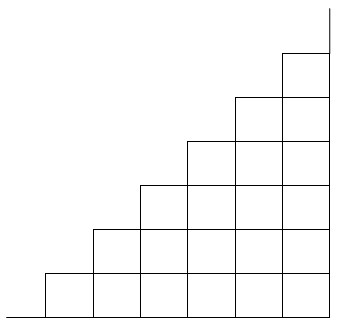
\includegraphics[scale=1]{09.jpg}

\end{figure}

\chapter{模型的求解}
我们将图补充完整
\begin{figure}[htbp]%位置选项
\centering
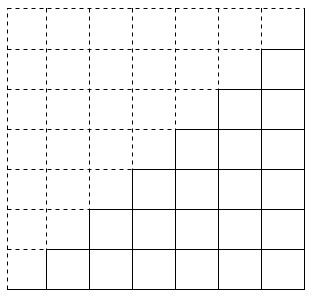
\includegraphics[scale=1]{1.jpg}
\end{figure}

考虑一个错误的走法,即路线越出了实线走到了虚线部分

\begin{figure}[htbp]%位置选项
\centering
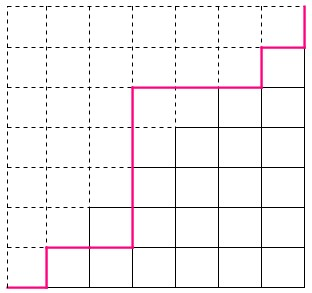
\includegraphics[scale=1]{2.jpg}
\end{figure}

我们找到超出实线边界的第一个点


\centering
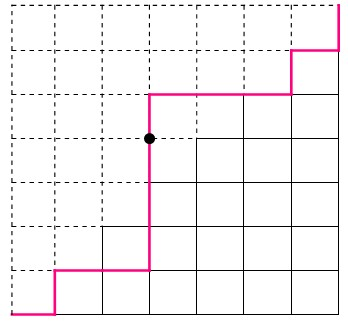
\includegraphics[scale=1]{2-2.jpg}



\flushleft
并以该点作出右上角部分的对称图形

\begin{figure}[htbp]%位置选项
\centering
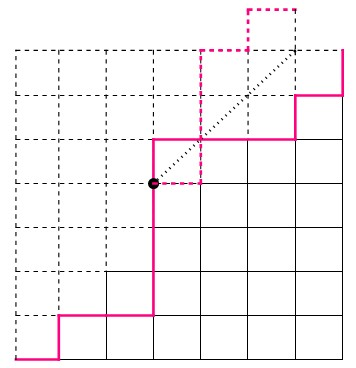
\includegraphics[scale=1]{3.jpg}
\end{figure}

这样我们就得到了一个由$(0,0)$到$(n-1,n+1)$的越界的路径,他由$n-1$次向右和$n+1$次向上运动组成.

考虑所有从$(0,0)$到$(n,n)$的移动,共有$\displaystyle\binom{2n}{n}$种走法,而所有越界的走法都可以对应为一个由$n-1$次向右和$n+1$次向上运动组成的走法,所以错误的走法数为$\displaystyle\binom{2n}{n-1}$,故总的正确走法数为
\[S_n=\binom{2n}{n}-\binom{2n}{n-1}=\frac{1}{n+1}\binom{2n}{n}\]



\chapter{程序的实现与结果测试}
我们首先通过一个搜索算法来枚举出1~n的全排列,将结果保存在数组target中,然后再调用test函数判断此序列是否是合法的出站序列.

\section{主要功能函数}
\subsection{全排列的枚举}
\begin{verbatim}
void dfs(int cur, int depth)//深度优先搜索
{
    if(cur == depth)
    {
#ifdef TEST
        for(int i = 1; i <= depth; i++)
            cout<<target[i];

        if(test(target, depth))
            cout<<" "<<"yes";
        else
            cout<<" "<<"no";
        cout<<endl;
#endif
        if(test(target, depth)) num++;

    }
    else
    {
        for(int i = 1; i <= depth; i++)
        {
            if(vis[i]) continue;
            vis[i] = 1;
            target[cur+1] = i;
            dfs(cur+1, depth);
            vis[i] = 0;
        }
    }
}

\end{verbatim}
\subsection{序列的判断}
\begin{verbatim}
bool test(int *target, int depth)
{
    stack<int> s;

    int a = 1,b = 1;
    while(b <= depth)
    {
        if(a == target[b]) {a++; b++;}

        else if(!s.empty() && s.top() == target[b]) {s.pop();b++;}

        else if(a <= depth) {s.push(a++);}

        else {return false;}
    }
    return true;
}
\end{verbatim}





\section{测试结果及分析}
首先给出的是在$n=3$和$n=4$时的测试情况,运行结果给出了每一种序列是否是合法序列.\\
\centering
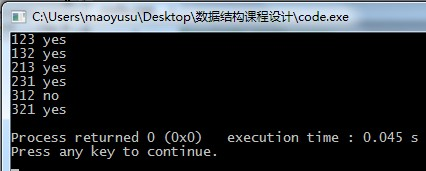
\includegraphics[scale=1]{a2.jpg}
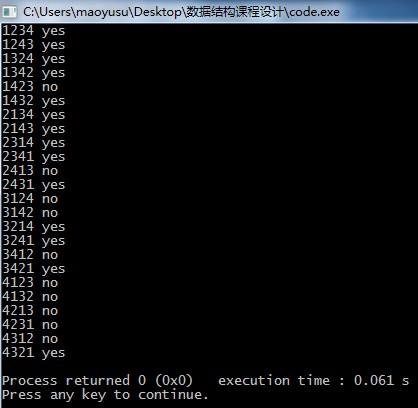
\includegraphics[scale=1]{a3.jpg}

\flushleft
然后我们测试$n=1$到$10$时,对应的出站序列总数,我们发现与所求通项是吻合的.

\centering
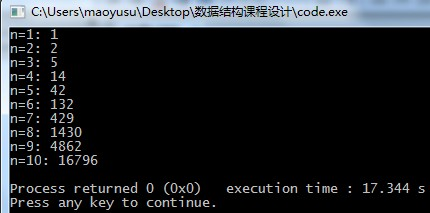
\includegraphics[scale=1]{a1.jpg}




\chapter{总结和问题}
\flushleft
  大二一年的学习,我们掌握了更多的编程的知识,也学习了更多的学科,这次的课题设计,不仅是不同学科之间的碰撞和交融,更是所学知识得以综合利用的一种体现,是自身综合能力的一次检验和锻炼,能有效的将所学的知识运用到实际,将不同的学科联系在一起,达到解决相关实际问题的目的。通过相关知识理论的了解和学习,终于设计出一种比较实际而又简洁的程序,很好的解决了二部图最大匹配问题。虽然这个计算程序已开发完成了,它也实现了我们所要解决的问题,但它仍有许多需要改进的地方。
\begin{enumerate}
	\item 程序运行效率不高,搜索算法的复杂度太大,不知可否优化.
	\item 我们所求得的数列为catalon数列,还有许多方法(比如生成函数法)可以求出它的通项,有待学习和扩充.
\end{enumerate}



\begin{thebibliography}{123}
\bibitem{WSHlssxyl}
	许胤龙. 组合数学引论(第2版) [M]. 合肥:中国科学技术大学出版社, 2010.
\bibitem{WSHlssxyls}
	knuth. 具体数学:计算机科学基础 [M]. 北京:人民邮电出版社, 2013
\bibitem{WSHlssxyl}
	刘汝佳. 算法竞赛入门经典 [M]. 北京:清华大学出版社, 2009
\end{thebibliography}
\acknowledgment
\hspace{\parindent}
  一份课程设计的总结,一份对老师的感谢。首先,必须感谢江老师的悉心教导;过去的几个学期,正是因为有您这样兢兢业业的老师,我们才可以在稳步的迈进程序设计的大门,正是由于您的认真负责,我们才可以在这个贪玩的年龄里,在这个易受外物影响的年龄里能够很好的学到应该掌握的知识,能够很好的将学到的运用于实际;

其次,必须感谢为了这份课程设计奉献过自己努力和给予帮助的同学,正是这份友谊,这份合作,我们才可以将这份课题设计圆满的完成,能够在这份设计中感受到友谊,同时也使自己得到相应的锻炼。
谢谢身边的每一个给予帮助的人,感谢生命中每一个孜孜奉献的每一个人,正是因为你们,所以我在这儿,健康而幸福的活着。
\clearpage
\phantomsection

\addcontentsline{toc}{chapter}{附录:程序代码}



\chapter*{附录:程序代码}
\begin{verbatim}
#include <iostream>
#include <stack>
using namespace std;
int vis[11], target[11];
int num;
bool test(int *target, int depth)
{
    stack<int> s;

    int a = 1,b = 1;
    while(b <= depth)
    {
        if(a == target[b]) {a++; b++;}

        else if(!s.empty() && s.top() == target[b]) {s.pop();b++;}

        else if(a <= depth) {s.push(a++);}

        else {return false;}
    }
    return true;
}
void dfs(int cur, int depth)
{
    if(cur == depth)
    {
#ifdef TEST
        for(int i = 1; i <= depth; i++)
            cout<<target[i];

        if(test(target, depth))
            cout<<" "<<"yes";
        else
            cout<<" "<<"no";
        cout<<endl;
#endif
        if(test(target, depth)) num++;

    }
    else
    {
        for(int i = 1; i <= depth; i++)
        {
            if(vis[i]) continue;
            vis[i] = 1;
            target[cur+1] = i;
            dfs(cur+1, depth);
            vis[i] = 0;
        }
    }
}

int main()
{
    for(int i = 1; i <= 10; i++)
    {
        num = 0;
        dfs(0,i);
        cout<<num<<endl;
    }
    return 0;
}

\end{verbatim}
\end{document}
